% Compilação isolada da seção de método (pdflatex + bibtex).
% latexmk -pdf preview.tex
\documentclass[10pt]{article}
\usepackage[margin=2.2cm]{geometry}
\usepackage[T1]{fontenc}

\usepackage{amsmath,amssymb,amsthm}
\usepackage{booktabs}
\usepackage{graphicx}
\usepackage{tikz}
\usetikzlibrary{arrows.meta,positioning,fit,backgrounds,shapes.geometric,calc}
\usepackage{algorithm}
\usepackage{algpseudocode}
\usepackage[hidelinks]{hyperref}
\newtheorem{proposition}{Proposition}
\title{WitnessRAG: Just-in-Time Witness Composition for Long-Term Agent Memory\\
\large Method and experimental design (draft)}
\author{}
\date{}
\begin{document}
\maketitle
% =====================================================================
% WitnessRAG -- Method and Experimental Design
% Drop-in section for the paper. Requires: amsmath, amssymb, amsthm,
% booktabs, tikz (arrows.meta, positioning, fit, backgrounds, calc,
% shapes.geometric),
% algorithm, algpseudocode. Citation keys are in witnessrag.bib.
% Every quantity below corresponds to code in the repository; the
% mapping is listed in docs/witnessrag-metodo.md (Section 10).
% =====================================================================

\section{WitnessRAG}\label{sec:method}

Long-term agent memory is usually built \emph{ahead of time}: histories are
compressed into summaries or graphs and requests are served from that
compressed store, which loses information that a later request may need.
General Agentic Memory (GAM)~\cite{yan2025gam} instead follows a
\emph{just-in-time} principle: an offline \emph{memorizer} keeps the full
history in a page store, and an online \emph{researcher} plans, searches,
integrates and reflects until the collected information suffices.
WitnessRAG keeps this division of labour but changes what the researcher
produces and how it decides it is done. Instead of a free-form integrated
summary judged sufficient by a language model, the researcher tries to
assemble a \emph{witness}: a minimal set of stored facts that, taken together,
entail an answer. Whether such a witness exists is decided by a symbolic join
over the fact memory, not by a further model call.

Three principles guide the design.
\textbf{(P1) Plan before searching}: a single planning call describes the
information need in a closed, task-agnostic vocabulary; no benchmark label is
ever consulted.
\textbf{(P2) Certify what can be certified}: questions whose answer is a
conjunction of stored facts are composed and checked against the memory;
questions outside that fragment are served by retrieval and specialised
signals.
\textbf{(P3) Intervene within bounds}: every intervention edits a fixed number
of positions of a strong hybrid context, so an error of the planner or of the
executor has a bounded cost.

% ---------------------------------------------------------------------
\subsection{Problem formulation}\label{sec:problem}

A history is a sequence of sessions $H=(s_1,\dots,s_T)$. Each turn $u$ has a
speaker, a text and a reference time $\tau(u)$, the date of its session.
The memorizer turns $H$ into a memory $\mathcal{M}$; for a question $q$ the
researcher returns a context $C(q)\subseteq\mathcal{P}$ of exactly $k$ pages,
and a reader produces $\hat a=\mathrm{Read}(q,C(q))$. As in GAM, the objective
is task performance under a fixed context budget,
\begin{equation}
  C^\star(q)\in\arg\max_{C\subseteq\mathcal{P},\,|C|=k}
  \;\mathbb{E}\bigl[\Gamma(\mathrm{Read}(q,C))\bigr],
  \label{eq:objective}
\end{equation}
where $\Gamma$ is the task metric; we additionally bound the number of online
model calls per question (Section~\ref{sec:cost}).

\paragraph{Queries and witnesses.}
A positive conjunctive query~\cite{chandra1977conjunctive} with answer
variable $x$ is
\begin{equation}
  Q(x)\;=\;\exists\,\bar y\;\bigwedge_{j=1}^{m} r_j(t_j, t'_j),
  \label{eq:cq}
\end{equation}
where each term is a constant or a variable. Given a fact base $F$ and an
answer $a$, the witnesses of $a$ are the inclusion-minimal subsets that entail
$Q(a)$:
\begin{equation}
  \mathcal{W}_{Q,a}=\bigl\{\,W\subseteq F \;:\; W\models Q(a),\;
  \forall W'\subsetneq W,\;W'\not\models Q(a)\bigr\}.
  \label{eq:witness}
\end{equation}
For any retained memory $S\subseteq F$, $a\in\mathrm{Ans}(Q,S)$ if and only if
some $W\in\mathcal{W}_{Q,a}$ satisfies $W\subseteq S$. Preserving and retrieving
answers therefore reduces to preserving and retrieving witnesses; the
witnesses of $a$ are the monomials of its provenance
polynomial~\cite{green2007provenance}. A one-atom
query ($m=1$) has one-fact witnesses; its witness is a single page, which a
retriever already approximates. Composition matters when $m\ge2$ or when the
answer is the \emph{set} of all $a$ with a witness.

% ---------------------------------------------------------------------
\subsection{Overview}\label{sec:overview}

\begin{figure*}[t]
\centering
\resizebox{\textwidth}{!}{%
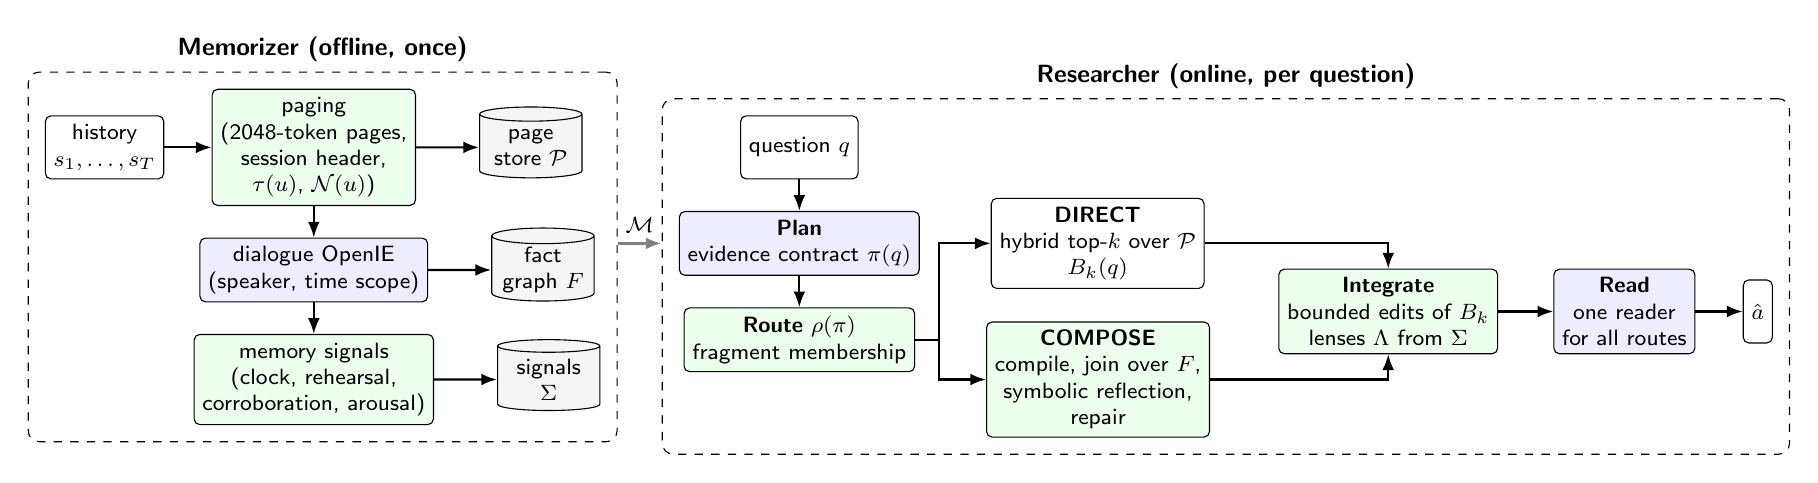
\begin{tikzpicture}[
  font=\sffamily\footnotesize, node distance=4mm and 6mm,
  box/.style={draw, rounded corners=2pt, align=center, minimum height=8mm,
              inner sep=3pt, fill=white},
  store/.style={draw, cylinder, shape border rotate=90, aspect=0.18,
                minimum height=9mm, minimum width=13mm, align=center,
                inner sep=1pt, fill=gray!8},
  llm/.style={box, fill=blue!7},
  sym/.style={box, fill=green!7},
  arr/.style={-{Latex[length=2mm]}, thick},
  grp/.style={draw, dashed, rounded corners=4pt, inner sep=6pt},
]
% ---------------- memorizer -----------------
\node[box] (hist) {history\\$s_1,\dots,s_T$};
\node[sym, right=of hist] (page) {paging\\(2048-token pages,\\session header,\\$\tau(u)$, $\mathcal{N}(u)$)};
\node[llm, below=of page] (ie) {dialogue OpenIE\\(speaker, time scope)};
\node[sym, below=of ie] (sig) {memory signals\\(clock, rehearsal,\\corroboration, arousal)};
\node[store, right=8mm of page] (P) {page\\store $\mathcal{P}$};
\node[store, right=8mm of ie] (F) {fact\\graph $F$};
\node[store, right=8mm of sig] (S) {signals\\$\Sigma$};
\draw[arr] (hist) -- (page);
\draw[arr] (page) -- (P);
\draw[arr] (page) -- (ie);
\draw[arr] (ie) -- (F);
\draw[arr] (ie) -- (sig);
\draw[arr] (sig) -- (S);
\begin{scope}[on background layer]
  \node[grp, fit=(hist)(page)(ie)(sig)(P)(F)(S), label={[font=\sffamily\small\bfseries]above:Memorizer (offline, once)}] (mem) {};
\end{scope}
% ---------------- researcher -----------------
\node[box, right=20mm of P] (q) {question $q$};
\node[llm, below=of q] (plan) {\textbf{Plan}\\evidence contract $\pi(q)$};
\node[sym, below=of plan] (route) {\textbf{Route} $\rho(\pi)$\\fragment membership};
\node[box, right=9mm of plan] (direct) {\textbf{DIRECT}\\hybrid top-$k$ over $\mathcal{P}$\\$B_k(q)$};
\node[sym, right=9mm of sig -| route.east, anchor=west] (compose) {\textbf{COMPOSE}\\compile, join over $F$,\\symbolic reflection,\\repair};
\coordinate (mid) at ($(direct.east)!0.5!(compose.east)$);
\node[sym, anchor=west] (integ) at ($(mid)+(9mm,0)$) {\textbf{Integrate}\\bounded edits of $B_k$\\lenses $\Lambda$ from $\Sigma$};
\node[llm, right=7mm of integ] (read) {\textbf{Read}\\one reader\\for all routes};
\node[box, right=6mm of read] (ans) {$\hat a$};
\draw[arr] (q) -- (plan);
\draw[arr] (plan) -- (route);
\draw[arr] (route.east) -- ++(3mm,0) |- (direct.west);
\draw[arr] (route.east) -- ++(3mm,0) |- (compose.west);
\draw[arr] (direct.east) -| (integ.north);
\draw[arr] (compose.east) -| (integ.south);
\draw[arr] (integ) -- (read);
\draw[arr] (read) -- (ans);
\begin{scope}[on background layer]
  \node[grp, fit=(q)(plan)(route)(direct)(compose)(integ)(read)(ans), label={[font=\sffamily\small\bfseries]above:Researcher (online, per question)}] (res) {};
\end{scope}
\draw[arr, very thick, gray] (mem.east |- plan) -- node[above, black] {$\mathcal{M}$} (res.west |- plan);
\end{tikzpicture}}
\caption{WitnessRAG. The memorizer keeps every turn in a page store and
derives a fact graph and memory signals. For each question the researcher
writes an evidence contract, routes by fragment membership, composes
witnesses when the need is conjunctive, edits a bounded number of positions of
the hybrid context, and calls a single reader. Blue: model calls; green:
symbolic, model-free steps.}
\label{fig:overview}
\end{figure*}

Figure~\ref{fig:overview} shows the two stages. Offline, the memorizer builds
$\mathcal{M}=\langle\mathcal{P},F,\tau,\Sigma\rangle$: pages, facts, the
reference clock and memory signals. Online, the researcher executes
\textsc{Plan}, \textsc{Route}, \textsc{Compose} (only when routed),
\textsc{Integrate} and \textsc{Read} (Algorithm~\ref{alg:researcher}).
Compared with GAM's plan--search--integrate--reflect loop, the plan also
selects memory signals, the reflection step is a symbolic closure test, and
integration is an edit of a retrieval context rather than a generated summary.

% ---------------------------------------------------------------------
\subsection{Memorizer: a witness-ready memory}\label{sec:memorizer}

\paragraph{Paging.}
The history is segmented into pages of at most 2{,}048 tokens, as in GAM's
page store. Each page starts with its session header, and every turn carries
its reference time $\tau(u)$. A deterministic normaliser $\mathcal{N}$ maps
relative expressions to absolute values anchored at $\tau(u)$
(``yesterday'' $\mapsto \tau(u)-1$ day; ``last week'' $\mapsto$ the
calendar week before $\tau(u)$), stored beside the original turn. No question,
answer or annotation is read.

\paragraph{Fact graph.}
A two-step extractor (entities, then triples) reads windows of 512 tokens with
64 tokens of overlap and emits at most 40 facts per window. A dialogue-aware
prompt resolves first-person speech to the speaker, scopes unnamed relatives
by their owner and attaches a time scope. Each fact is
$f=(s,r,o,p,t,c)$: subject, relation, object, source page, time and confidence
($c=0.9$ for a single extraction). Entities are grouped into canonical
identity clusters (lexical containment confirmed by embedding similarity
$\ge0.80$) and relations into morphological families, so that a join is not
broken by spelling variants. Entities, relations, facts and pages are
embedded with BGE-M3~\cite{chen2024bgem3}. The same fact base is shared with
every graph baseline.

\paragraph{Memory signals.}
Three model-free statistics are computed once:
the reference clock $[t_0,t_{\text{now}}]$ (first and last session);
the \emph{rehearsal} count $n(s,r)$, the number of pages that restate a fact
with the same canonical subject and relation; and the \emph{corroboration}
count $m(f)$, the number of extractions that support the same canonical
triple. Emotional arousal $\alpha(u)$ of each turn is computed on demand
(Section~\ref{sec:lenses}).

% ---------------------------------------------------------------------
\subsection{Plan: the evidence contract}\label{sec:contract}

The researcher first describes \emph{what} the question needs, before any
search. One model call maps the question text to an evidence contract
\begin{equation}
  \pi(q)=\langle \phi,\;\omega,\;\sigma,\;\theta,\;E,\;N,\;\Lambda\rangle,
  \label{eq:contract}
\end{equation}
with a closed vocabulary:
the answer form $\phi\in\{$entity, set, count, time, duration, yes/no, choice,
description$\}$;
the reasoning operator $\omega\in\{$lookup, aggregate, join, compare,
temporal, abduce$\}$;
the evidence scope $\sigma\in\{$single, multiple$\}$, i.e.\ whether a complete
answer needs statements recorded in more than one place or occasion;
the temporal focus $\theta=(\text{focus},\text{anchor})$;
focus entities $E$; up to four information needs $N$, which play the role of
GAM's info-needs; and the memory lenses $\Lambda$ that should re-rank evidence
(Section~\ref{sec:lenses}).
The planner receives only the question: no memory content, no gold answer,
no supporting passage and no benchmark category. Outputs outside the
vocabulary are normalised through a fixed alias table or rejected; an invalid
or content-filtered contract is written $\pi=\bot$.

% ---------------------------------------------------------------------
\subsection{Route: fragment membership}\label{sec:route}

The route is a deterministic function of the contract, derived from what the
witness executor can certify:
\begin{equation}
  \rho(\pi)=
  \begin{cases}
    \textsc{Compose} & \text{if } \omega\in\{\text{aggregate},\text{join},\text{compare}\}
      \;\wedge\; \sigma=\text{multiple}\\
      & \;\wedge\; \phi\in\{\text{entity},\text{set},\text{count},\text{description}\},\\
    \textsc{Direct} & \text{otherwise, including } \pi=\bot.
  \end{cases}
  \label{eq:route}
\end{equation}
The executor proves positive conjunctive queries whose answer variable ranges
over entities (Eq.~\ref{eq:cq}). A lookup is a one-atom query, which a
retriever already serves. Temporal arithmetic, abduction (``would'',
``likely'') and truth-valued answers lie outside the executable fragment and
are served by the temporal memory and the reader. The route is therefore not a
question-type classifier: it asks whether the need belongs to the fragment in
which a witness can exist. Unlike Adaptive-RAG~\cite{jeong2024adaptiverag},
which trains a classifier of question complexity, it needs no labelled
training questions.

Let $\rho_{\mathcal{L}}(q)$ denote the route of a controller that reads a
benchmark label (e.g.\ compose iff the question is annotated as multi-hop).

\begin{proposition}[Route equivalence]\label{prop:equivalence}
Assume deterministic decoding or a shared response cache, and lenses disabled.
If $\rho(\pi(q))=\rho_{\mathcal{L}}(q)$, then WitnessRAG and the labelled
controller produce the same context and the same answer for $q$. Consequently,
for any metric $\Gamma\in[0,1]$ averaged over $N$ questions,
\begin{equation}
  \bigl|\bar\Gamma_{\text{WitnessRAG}}-\bar\Gamma_{\mathcal{L}}\bigr|
  \;\le\; \frac{|D_{\text{eff}}|}{N}
  \;\le\; \frac{\bigl|\{q:\rho(\pi(q))\neq\rho_{\mathcal{L}}(q)\}\bigr|}{N},
  \label{eq:bound}
\end{equation}
where $D_{\text{eff}}$ is the set of disagreeing questions on which at least one
controller edits the hybrid context.
\end{proposition}
\begin{proof}[Sketch]
Both controllers call the same \textsc{Compose} and \textsc{Direct} procedures
with the same arguments; the compiler prompt depends on $q$ and on the graph
vocabulary only, and the reader prompt on $q$ and $C(q)$ only. On an agreeing
question every call is identical. On a disagreeing question in which neither
controller edits $B_k(q)$ the contexts coincide as well. The bound follows
from $\Gamma\in[0,1]$.
\end{proof}

The right-hand side of Eq.~\ref{eq:bound} can be measured with one planning
call per question, before any full run.

% ---------------------------------------------------------------------
\subsection{Compose: witness search with symbolic reflection}\label{sec:compose}

\paragraph{Compilation.}
A second call compiles $q$ into a conjunctive query $Q$ (Eq.~\ref{eq:cq}) with
at most four atoms, an answer variable and an aggregation in
$\{$none, set, count$\}$. The prompt lists, as suggestions, the 40 relations
and 20 entities of the graph closest to $q$ in embedding space, which prevents
predicates that no fact instantiates.

\paragraph{Grounding.}
An atom $a=r(t,t')$ is matched to a fact $f$ with score
\begin{equation}
  g(a,f)=\frac{w_r\,\mathrm{sim}(r,r_f)+w_c\,\mathrm{sim}_{\text{const}}(a,f)
  +w_v\,\mathrm{sim}(\mathrm{verb}(a),\mathrm{verb}(f))}{w_r+w_c+w_v},
  \label{eq:grounding}
\end{equation}
with $(w_r,w_c,w_v)=(0.45,0.35,0.20)$ and a hard threshold
$\mathrm{sim}(r,r_f)\ge0.65$. Each constant is linked to at most five
canonical identity clusters with similarity $\ge0.55$ (an exact match scores
$1$); a fact is admissible only if its argument lies in one of them, and
$\mathrm{sim}_{\text{const}}$ is that linking similarity ($w_c$ is dropped when
the atom has no constant). Relation direction is never inverted by
similarity: an inverse relation must be a different explicit predicate. After
a variable is bound, its neighbourhood is re-grounded (binding-aware
grounding), and each atom keeps at most 60 candidates.

\paragraph{Join.}
A beam search (width 400) extends partial assignments atom by atom, most
constrained first, and keeps an assignment only if every shared variable
receives the same canonical cluster. Complete assignments yield
inclusion-minimal witnesses $W$ with
$\mathrm{score}(W)=\prod_{f\in W}g(a_f,f)$ and support
\begin{equation}
  \mathrm{supp}(a)=\max_{W\in\widehat{\mathcal{W}}_{Q,a}}\;
  \mathrm{score}(W)\prod_{f\in W}c_f,
  \label{eq:support}
\end{equation}
which does not grow when a proof is duplicated. Answers are grouped by
canonical symbol; with aggregation \emph{set} or \emph{count}, the answer is
the set of witnessed assignments.

\paragraph{Symbolic reflection.}
Where GAM asks a model whether the integrated information is sufficient,
WitnessRAG tests sufficiency on the join itself:
\begin{equation}
  y(q)=\mathbf{1}\Bigl[\,\widehat{\mathcal{W}}\neq\emptyset
  \wedge |A|\le 3 \wedge |\widehat{\mathcal{W}}|\le 3
  \wedge \text{no truncation}
  \wedge \mathrm{supp}(a_1)\ge 0.45
  \wedge \bigl|\mathrm{pages}(W^\star)\bigr|\le 2\Bigr],
  \label{eq:reflection}
\end{equation}
where $A$ is the answer set, $a_1$ its best-supported answer and $W^\star$
the witnesses selected for insertion. If $Q$ has fewer than two connected atoms
or a non-executable aggregation, the join is skipped and $y(q)=0$. A broad
answer set, many duplicate proofs or a truncated search signal that the plan
is not selective, and the witness is not allowed to displace retrieved
evidence. When $y(q)=1$, whole witnesses (never partial ones) enter the tail
of the context.

\paragraph{Repair.}
When $y(q)=0$, the failure is turned into at most one follow-up search, the
analogue of GAM's follow-up request $r'$:
(i)~\emph{agreement probes}: the compiled keyword query and the verbalised
atoms (at most four) are issued as independent searches; a page enters only
if at least two probes retrieve it within their top ten, outside the protected
prefix;
(ii)~\emph{gap-directed probe}: if the join stopped at an atom with a bound
entity $e$ and a missing relation $r$, the probe ``$e\ r$'' is issued and the
first new page that literally mentions $e$ is admitted.
Repairs are recorded as hypotheses, never as proofs.

% ---------------------------------------------------------------------
\subsection{Memory lenses}\label{sec:lenses}

The Bridging Reflective and Semantic Memory architecture~\cite{flexa2026bridging}
scores a memory item by relevance, temporal stability and affectivity,
$\mathrm{Score}_i=R_i\,[\beta S_i+(1-\beta)A_i]$, and Generative
Agents~\cite{park2023generative} combine recency, importance and relevance;
both use the same weights for every request. WitnessRAG turns these signals into \emph{lenses} that the
contract switches on per question. For a candidate page $p$ in the hybrid pool,
\begin{equation}
  s(p\mid q,\pi)=\tilde R(p,q)\,\Bigl(1+\beta\sum_{\ell\in\Lambda}\Phi_\ell(p\mid q,\pi)\Bigr),
  \label{eq:lens-score}
\end{equation}
where $\tilde R$ is the hybrid relevance min--max normalised over the pool.
Relevance stays multiplicative, so an irrelevant memory is never promoted by
being recent or emotional. Let $F_E(p)$ be the facts of $p$ about the focus
entities and $\mathcal{T}(p)$ the reference times of $p$ (session dates,
normalised event dates and fact times).

\paragraph{Temporal lens.}
With the reference clock $[t_0,t_{\text{now}}]$ and anchor interval $I$ parsed
from $\theta$,
\begin{equation}
  \Phi_T(p)=
  \begin{cases}
   \max_{t\in\mathcal{T}(p)}\exp\!\bigl(-(t_{\text{now}}-t)/s_p\bigr),
     & \text{recent},\\
   \exp\!\bigl(-(\min\mathcal{T}(p)-t_0)/s_0\bigr), & \text{early},\\
   \max_{t\in\mathcal{T}(p)}\exp\!\bigl(-d(t,I)/w_I\bigr), & \text{anchor},
  \end{cases}
  \qquad s_p=s_0+\alpha\bigl(\max_{f\in F_E(p)}n(s_f,r_f)-1\bigr),
  \label{eq:temporal}
\end{equation}
where $d(t,I)$ is the distance in days from $t$ to $I$ and
$w_I=\max(7,|I|/2)$. The \emph{recent} case is the Ebbinghaus retention of the
architecture in~\cite{flexa2026bridging}, $S=\exp(-\Delta t/s)$ with
$s=s_0+\alpha n$; here $n$ counts rehearsals in the dialogue (a fact restated
across sessions decays more slowly), the conversational analogue of repeated
retrieval. We use $s_0=\alpha=30$ days.

\paragraph{Salience lens.}
Emotionally arousing experiences are consolidated preferentially in human
memory~\cite{mcgaugh2004amygdala}. For turns $u$ of $p$ spoken by, or
mentioning, a focus entity,
\begin{equation}
  \Phi_A(p)=\max_{u}\;\bigl(1-e^{-\epsilon(u)/\kappa}\bigr)\cdot
  \Bigl(\tfrac12+\tfrac12\min\bigl(1,\tfrac{|\mathrm{terms}(u)\cap\mathrm{terms}(q)|}{2}\bigr)\Bigr),
  \label{eq:salience}
\end{equation}
where $\epsilon(u)$ sums arousal-lexicon weights, intensifiers and
exclamations, and $\kappa=2$. In~\cite{flexa2026bridging} affectivity is a
utility learned from reflective feedback, $A_i(t+1)=A_i(t)+\lambda_i(t)$. No
such feedback is available when a test set is answered, and cross-question
updates would make answers depend on question order. $\Phi_A$ is therefore
the \emph{prior} of affectivity; in a lifelong deployment the natural
utility signal is witness participation, $\lambda_f=+1$ when $f$ belongs to a
delivered witness of a confirmed answer.

\paragraph{Confidence lens.}
Confidence is epistemic, not affective: it measures whether a statement is
reliably recorded, not whether it matters to the person. Treating repeated
extractions as independent evidence,
\begin{equation}
  \Phi_C(p)=\max_{f\in F_E(p)}\;\bigl(1-(1-c_f)^{m(f)}\bigr)\cdot
  \max\bigl(0,\cos(e(N),e(f))\bigr),
  \label{eq:confidence}
\end{equation}
where $e(N)$ is the mean embedding of the contract's information needs.

\paragraph{Lens integration.}
Lenses compete only for the unprotected tail. A candidate $p^+$ replaces the
weakest tail page $p^-$ only if its lens gain is larger,
$\sum_\ell\Phi_\ell(p^+)>\sum_\ell\Phi_\ell(p^-)$, and
$s(p^+)>(1+\delta)\,s(p^-)$ with $\delta=0.1$, for at most $L$ swaps
($L=1$ by default). Pages placed by \textsc{Compose} are protected. Without an
active lens the procedure is the identity.

% ---------------------------------------------------------------------
\subsection{Integrate and read}\label{sec:integrate}

Let $B_k(q)$ be the hybrid context: dense and BM25 rankings fused by
reciprocal rank fusion~\cite{cormack2009rrf} ($k_{\text{rrf}}=60$) over a pool
of 20 pages, truncated to $k=5$. All interventions are edits of $B_k$ with a
protected prefix: a witness may replace the last two positions, an agreed or
gap-directed probe the last one, and lenses at most $L$ unprotected positions.
Hence
\begin{equation}
  |C(q)\setminus B_k(q)|\le\max(2,L),
  \label{eq:edits}
\end{equation}
and the first $k-\max(2,L)$ hybrid pages are always delivered. A single
reader serves every route and every baseline: one call that identifies the
requested operation (entity, option, inference, list, distinct count, date,
interval or duration), reads a temporal view in which each turn carries
$\tau(u)$ and $\mathcal{N}(u)$, and returns a short span. Holding the reader
fixed makes differences between systems differences in retrieval.

\begin{algorithm}[t]
\caption{WitnessRAG researcher (one question)}\label{alg:researcher}
\begin{algorithmic}[1]
\Require question $q$, memory $\mathcal{M}=\langle\mathcal{P},F,\tau,\Sigma\rangle$, budget $k$
\State $(\mathcal{C},\,r)\gets\textsc{Hybrid}(q,\,20)$; \quad $B\gets\mathcal{C}[1{:}k]$
\State $\pi\gets\textsc{Plan}(q)$ \Comment{model call 1; question text only}
\State $C\gets B$
\If{$\rho(\pi)=\textsc{Compose}$} \Comment{Eq.~\ref{eq:route}}
  \State $Q\gets\textsc{Compile}(q,\,\mathrm{Vocab}(q,F))$ \Comment{model call 2}
  \State $\widehat{\mathcal W},A\gets\textsc{Join}(Q,F)$ \Comment{symbolic}
  \If{$y(q)=1$} \Comment{symbolic reflection, Eq.~\ref{eq:reflection}}
     \State $C\gets\textsc{Insert}(B,\mathrm{pages}(W^\star))$ \Comment{$\le2$ tail slots}
  \ElsIf{a page is retrieved by $\ge2$ probes of $Q$}
     \State $C\gets\textsc{Insert}(B,\text{that page})$ \Comment{1 tail slot}
  \ElsIf{the join exposes a gap $(e,r)$}
     \State $C\gets\textsc{Insert}(B,\textsc{Probe}(e\ r))$ \Comment{1 tail slot}
  \EndIf
\EndIf
\If{$\Lambda(\pi)\neq\emptyset$}
  \State $C\gets\textsc{Lenses}(C,\mathcal{C},r,\Lambda,\Sigma)$ \Comment{$\le L$ swaps, Eq.~\ref{eq:lens-score}}
\EndIf
\State \Return $\textsc{Read}(q,C)$ \Comment{final model call}
\end{algorithmic}
\end{algorithm}

% ---------------------------------------------------------------------
\subsection{Cost}\label{sec:cost}

Offline, the memorizer spends one entity call and one triple call per
extraction window; signals are model-free. Online, the number of model calls
is
\begin{equation}
  c(q)=\underbrace{1}_{\textsc{Plan}}+\underbrace{\mathbf{1}[\rho(\pi)=\textsc{Compose}]}_{\textsc{Compile}}
  +\underbrace{1}_{\textsc{Read}},
  \label{eq:cost}
\end{equation}
so $\mathbb{E}[c]=2+\Pr[\textsc{Compose}]$. There is no online extraction,
verification or re-planning. A GAM researcher with reflection depth three may
issue planning, integration, sufficiency and follow-up calls in every round.
A label-routed controller costs $1+\Pr[\text{multi-hop}]$ calls; the price of
not reading the label is exactly one planning call.

% =====================================================================
\section{Experimental design}\label{sec:experiments}

We follow the evaluation protocol of GAM~\cite{yan2025gam} and ask four
questions.
\textbf{RQ1}: does planning without category labels preserve the
effectiveness of a label-routed controller?
\textbf{RQ2}: how does WitnessRAG compare with memory-free, graph-based and
memory-based systems?
\textbf{RQ3}: what does each component contribute (routing, composition,
lenses)?
\textbf{RQ4}: what does it cost, and how does effectiveness change with the
edit budget?

\paragraph{Benchmarks.}
LoCoMo~\cite{maharana2024locomo}: the ten conversations, 1{,}540 questions of
categories 1--4 (single-hop, multi-hop, temporal, open-domain). Each
conversation is a separate memory. Categories are used \emph{only} to report
results and to evaluate routing. HotpotQA~\cite{yang2018hotpotqa} with memories
of 56K, 224K and 448K tokens built by adding seeded distractors to the gold
supports; RULER~\cite{hsieh2024ruler} at 128K tokens (retrieval, multi-hop
tracing, aggregation, QA); NarrativeQA~\cite{kocisky2018narrativeqa}.

\paragraph{Baselines.}
Memory-free: long-context LLM and RAG over 2{,}048-token pages (dense top-5,
as in GAM), BM25 and hybrid RRF. Graph-based, over the \emph{same} extracted
fact base: GraphRAG~\cite{edge2024graphrag}, HippoRAG~\cite{gutierrez2024hipporag}
and HippoRAG~2~\cite{gutierrez2025hipporag2}. Memory-based systems (A-Mem,
Mem0, MemoryOS, LightMem, GAM) are reported from~\cite{yan2025gam} and marked
as such, since backbones and extraction differ.

\paragraph{Metrics.}
LoCoMo: official token F1 and BLEU-1 per category; HotpotQA and NarrativeQA:
F1; RULER: accuracy per task. Retrieval: all-recall@5 against annotated
evidence. Faithfulness: rate of complete witnesses delivered in context.
Cost: model calls, prompt and completion tokens, and latency per question.
Routing (RQ1): agreement of $\rho(\pi)$ with the labelled route and the
effective disagreement $|D_{\text{eff}}|/N$ of Eq.~\ref{eq:bound}.

\paragraph{Arms.}
\begin{center}
\small
\begin{tabular}{@{}lll@{}}
\toprule
Arm & Routing & What it isolates \\
\midrule
Hybrid & none & strong retrieval baseline $B_k$ \\
Label-routed & benchmark label (privileged) & upper reference for routing \\
\textbf{WitnessRAG} & evidence contract & main system (RQ1, RQ2) \\
\quad + lenses & contract + $\Lambda$ & temporal, salience, confidence (RQ3) \\
\quad + one lens & contract + one $\ell$ & contribution of each lens \\
Compose-all & plan, then always \textsc{Compose} & value of routing \\
Direct-all & plan, then always \textsc{Direct} & planner overhead, value of composition \\
\bottomrule
\end{tabular}
\end{center}
For RQ4 we vary the lens budget $L\in\{1,2\}$, the analogue of GAM's number of
retrieved pages.

\paragraph{Statistical protocol and leakage control.}
All arms share the corpus, the extracted fact base, the embedder, the reader,
$k=5$, temperature $0$, seed $42$ and a response cache, so paired differences
isolate the method. We report question-level paired bootstrap confidence
intervals (5{,}000 resamples, 95\%). The planner and the compiler never see
answers, evidence annotations or categories. Controller thresholds were set
while developing on the first LoCoMo conversation; we therefore also report
the nine remaining conversations separately as a held-out check.

\paragraph{Implementation.}
Backbones: GPT-4.1-mini (Azure deployment) and Qwen2.5-14B-Instruct (vLLM),
the same model for memorizer, planner, compiler and reader; embeddings:
BGE-M3. Pages of 2{,}048 tokens; extraction windows of 512 tokens (overlap 64,
at most 40 triples); pool of 20 candidates; $k=5$; at most four atoms; 60
grounding candidates per atom; beam width 400; lens weight $\beta=1$,
$\delta=0.1$, $L=1$, $s_0=\alpha=30$ days.

\bibliographystyle{plain}
\bibliography{witnessrag}
\end{document}
